% !TEX root = master_thesis.tex
\chapter{Experimental Setup}
\label{chap:exp}
In this work the beam asymmetry $\Sigma$ is determined in the reactions $\gamma p\to p\eta$ and $\gamma p\to p\eta'$, requiring a polarized photon beam and an unpolarized proton target. It is convenient to study photoproduction off a fixed target and investigate the resonances that occur in the process. The analyzed data was taken at the CBELSA/TAPS experiment located in Bonn  at the ELectron Stretcher Accelerator (ELSA). In this chapter the different parts of the CBELSA/TAPS experiment that are used for the measurement of the beam asymmetry $\Sigma$ will be presented. Figure \ref{fig:cbarea} shows an overview of the experimental hall. All mentioned parts are discussed in detail in the following
\begin{figure}[htbp]
	\centering
	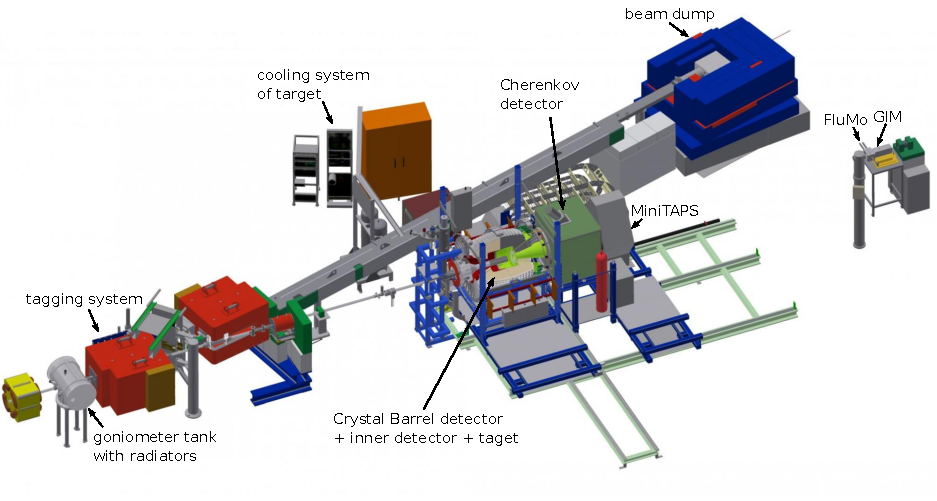
\includegraphics[width=\linewidth]{figs/cbarea.pdf}
	\caption{Overview of the experimental hall of the CBELSA/TAPS experiment. The electron beam from ELSA enters at the top right. \textsc{M. Grüner} in \cite{farahphd}}
	\label{fig:cbarea}
\end{figure}
\noindent High energy electrons extracted from ELSA are used to produce a polarized photon beam using the \emph{bremsstrahlung} process (see \ref{subsec:goni}). After they have been energy tagged (see \ref{subsec:tag}) these photons then interact with the fixed target material (see Section \ref{sec:tar}) so that hadronic resonances may be excited that will decay via the strong interaction under the emission of mesons. The resulting decay products can then be measured with a system of electromagnetic calorimeters and scintillators that is especially suited for the detection of photons (see Section \ref{sec:cal}). The analogue measurements are only saved for offline analysis if detector signals meet certain trigger conditions which is only the case for reactions that are of interest (see Section \ref{sec:trig}). This way the amount of unwanted background is minimized already during the process of data taking. Once data acquisition is finished the data may be investigated with the help of analysis software and Monte Carlo simulations tailored to the needs of the CBELSA/TAPS experiment (see Section \ref{sec:mc}).
\section{Production of polarized high energy photon beam}
\label{sec:pol}
To measure polarization observables in photoproduction reactions a polarized photon beam is needed which can be created using \emph{coherent bremsstrahlung}. Bremsstrahlung is the dominating interaction of high energy ($\mathcal{O}\left(\SI{1e0}{\giga\eV}\right)$) electrons with matter \cite{leo}. Electrons are decelerated in the \textsc{Coloumb} field of heavy nuclei and radiate real photons, see Figure \ref{fig:brems}. 

\begin{figure}[htbp]
	\centering
	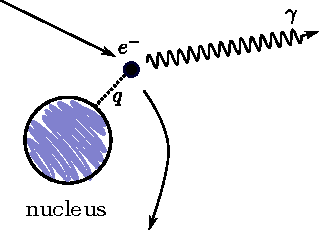
\includegraphics[width=.5\linewidth]{brems.pdf}
	\caption{Illustration of the bremsstrahlung process: An electron $e^-$ is deflected in the \textsc{Coloumb} field of a nucleus in the radiator material. A photon $\gamma$ is emitted and so the momentum $q$ is transferred.}
	\label{fig:brems}
\end{figure}
\noindent To conserve momentum there has to be a momentum transfer $q$ which is negligibly small compared to the nucleon mass. If an amorphous radiator is used incoherent bremsstrahlung is produced with a continuous spectral distribution proportional to $1/E_\gamma$ according to the \textsc{Bethe-Heithler} cross section \cite{hei}. Since the structure of nuclei in the amorphous radiator does not exhibit any periodicity, the electric field vector will not prefer any particular direction, resulting in a net polarization degree of zero for the photon beam. To achieve non-vanishing polarization degrees a crystal with periodic placement of nuclei may be used as radiator. Then, coherent bremsstrahlung is produced; the crystal can absorb the recoil only for discrete momenta $q_n$ meeting the \textsc{Laue} condition \cite{dem} of the crystal lattice. This enables constructive interference between different bremsstrahl photons and at the same time fixes the deflection plane of incoming electrons, resulting in a coherent polarized photon beam. Incoherent bremsstrahlung may still occur due to impurities in the crystal structure, so that the total bremsstrahlung cross section off a crystal radiator $\sigma_\text{crystal}$ is the sum of a coherent ($\sigma_\text{coherent}$) and an incoherent ($\sigma_\text{incoherent}$) part
\begin{equation}
	\sigma_\text{crystal}=\sigma_\text{coherent}+\sigma_\text{incoherent}.
\end{equation}
The process of bremsstrahlung can be modeled using ANalytical Bremsstrahlung (ANB) calculations \cite{anb}. ANB intensity spectra for a crystal and amorphous radiator are shown in Figure \ref{fig:anb} on the left hand side. The right hand side shows the enhancement spectrum, which is given by dividing the two spectra. 
\begin{figure}[htbp]
	\centering
	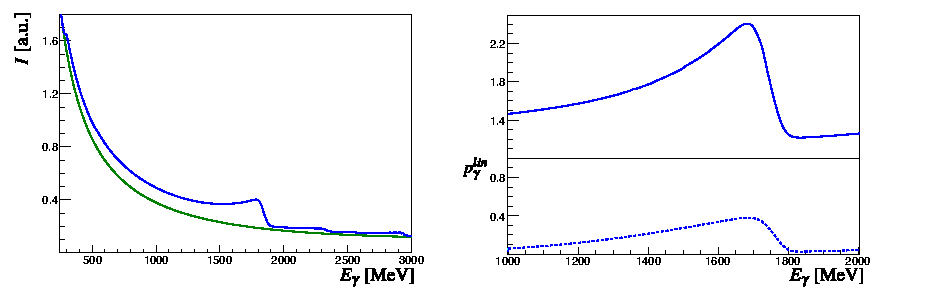
\includegraphics[width=\linewidth]{figs/anb.pdf}
	\caption{Left: Incoherent (green) and crystal (blue) bremsstrahlung intensities as a function of the photon energy. Right: The enhancement spectrum is given as the ratio of crystal to incoherent intensity spectrum. The dashed line at the bottom shows the calculated polarization degree. Both spectra are generated using ANB calculations. Taken from \cite{farahphd}.}
	\label{fig:anb}
\end{figure} 
One observes that the bremsstrahlung intensity spectrum obtained from a crystal radiator is in general enhanced relative to the incoherent spectrum obtained from an amorphous radiator. In fact, using ANB calculations, the polarization degree can be determined from the enhancement spectrum. The characteristic drop in intensity in the intensity spectrum obtained from the crystal radiator is referred to as the coherent edge. It occurs because the photon energy in the kinematically allowed region of the recoil momentum that will lead to coherent bremsstrahlung is limited. The relative alignment of the radiation crystal to the electron beam determines the position of the coherent edge. 
\subsection{Goniometer}
In order to determine the beam polarization from enhancement spectra, a diamond radiator as well as an amorphous radiator are required. Several radiators as well as beam diagnostics tools mounted inside a rotating aluminum wheel are part of the goniometer \cite{goni}, resting inside a vacuum tank. Depending on whether linearly polarized or unpolarized photons are needed either copper radiators of different thickness or a diamond radiator, which is located in the center of the wheel, are inserted into the beam axis, see Figure \ref{fig:goni}. In case a circularly polarized photon beam is required, a \textsc{M\o ller} polarimeter \cite{moller} is used, which is also shown in Figure \ref{fig:goni}. The goniometer can be rotated in all directions allowing precise alignment with the incoming electron beam from ELSA.  
\label{subsec:goni}

\subsection{Tagging system}
\label{subsec:tag}
Once the impinging electrons from ELSA have scattered off the radiator their energy is determined in order to measure the energy of the created photons. This is possible because the initial electron energy $E_0=\SI{3.2}{\giga\eV}$ is known from ELSA. Thus, the photon Energy $E_\gamma$ is given by subtracting the energy of the recoil electrons $E_e$ from $E_0$\footnote{Hereby, the recoil energy absorbed by the nuclei is neglected.} 
\begin{equation}
	E_\gamma=E_0-E_e.
\end{equation}
The recoiling electrons are deflected towards the tagging system \cite{tagger} consisting of 96 overlapping scintillator bars and 480 scintillating fibers using the magnetic field of a dipole magnet with a field strength of $\SI{1.5}{\tesla}$. The bending radius of the electrons depends on their momenta is uniquely defined by the tagger hit position. With the position of the deflected electrons and the magnetic field strength, $E_e$ can thus be determined. For an initial energy $E_0=\SI{3.2}{\giga\eV}$ the scintillator bars cover an energy range of $\SI{560}{\mega\eV}<E_\gamma<\SI{3100}{\mega\eV}$ with an energy resolution of $0.1\%E_\gamma$-$6\%E_\gamma$. The fibers additionally improve the energy resolution in the energy range $\SI{416}{\mega\eV}<E_\gamma<\SI{2670}{\mega\eV}$ to $0.1\%E_\gamma$-$0.4\%E_\gamma$. Photomultipliers are used for the readout of the tagger bars and fibers, realizing a time resolution of \footnote{Full Width Half Maximum.}$\text{FWHM}_\text{bar}=\SI{635}{\pico\s}$ and $\text{FWHM}_\text{fiber}=\SI{1.964}{\nano\s}$ \cite{hartmanndipl}. Any electrons that have not interacted with the radiator material are deflected by another dipole magnet towards the beam dump, see Figure \ref{fig:cbarea}. Figure \ref{fig:tagger} shows a top-down view of the tagging system.

\begin{minipage}[htbp]{.45\linewidth}
	\begin{figure}[H]
		\centering
		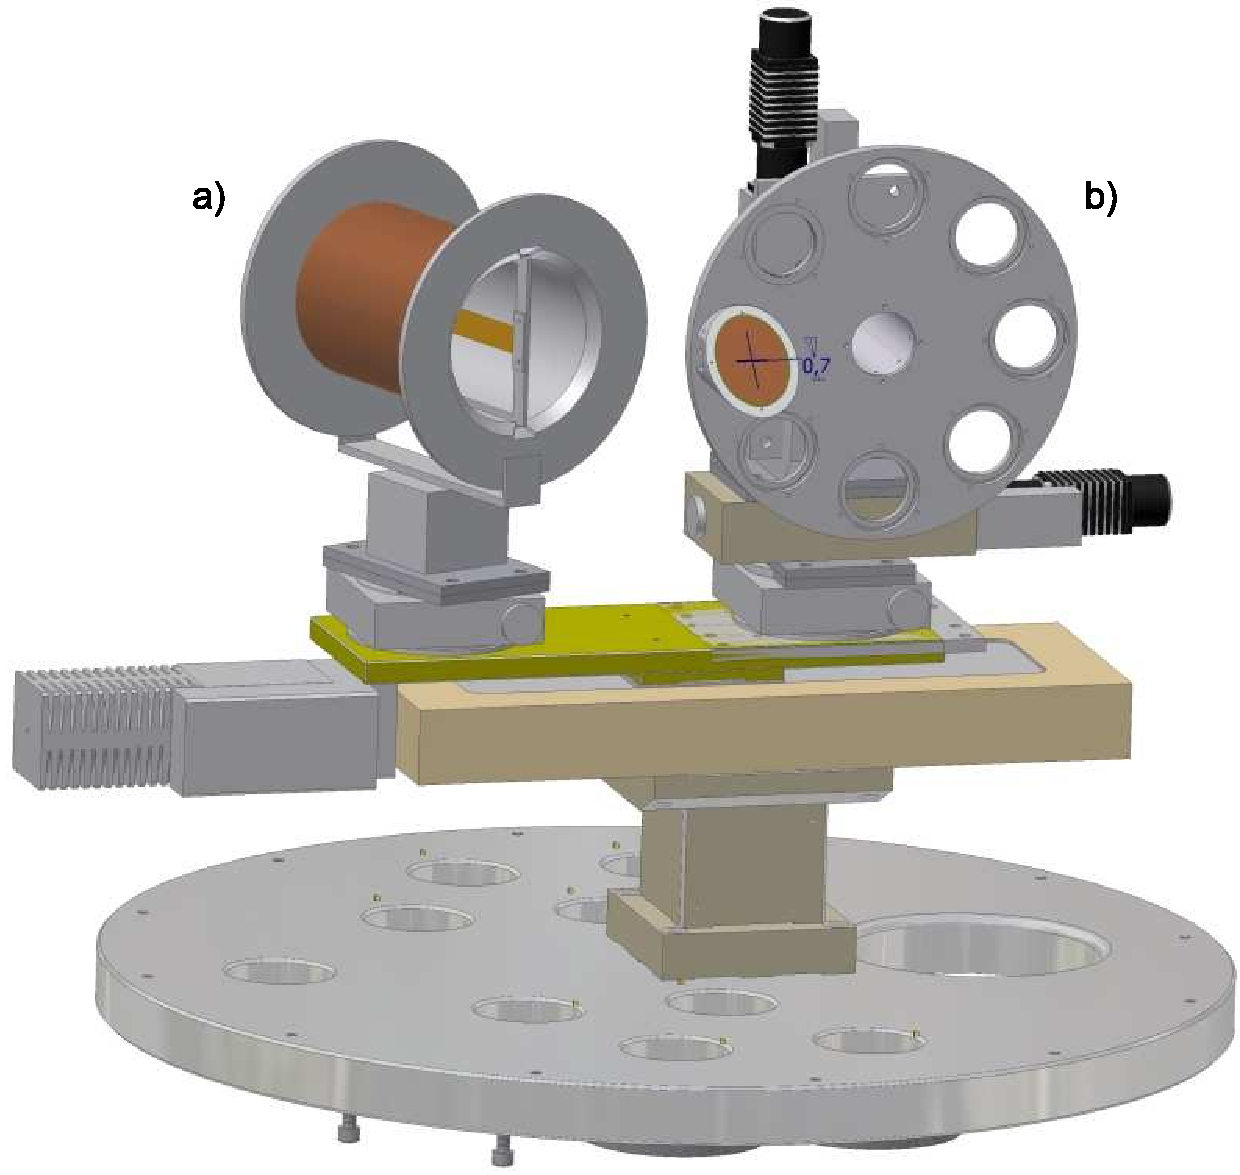
\includegraphics[width=\linewidth]{figs/goni-ganz.pdf}
		\caption{The goniometer holds several radiators that can be inserted onto the beam axis (b). Also available is a \textsc{M\o ller} radiator \cite{cb}.\\}
		\label{fig:goni}
	\end{figure}
\end{minipage}
\hfill
\begin{minipage}[htbp]{.49\linewidth}
\begin{figure}[H]
	\centering
	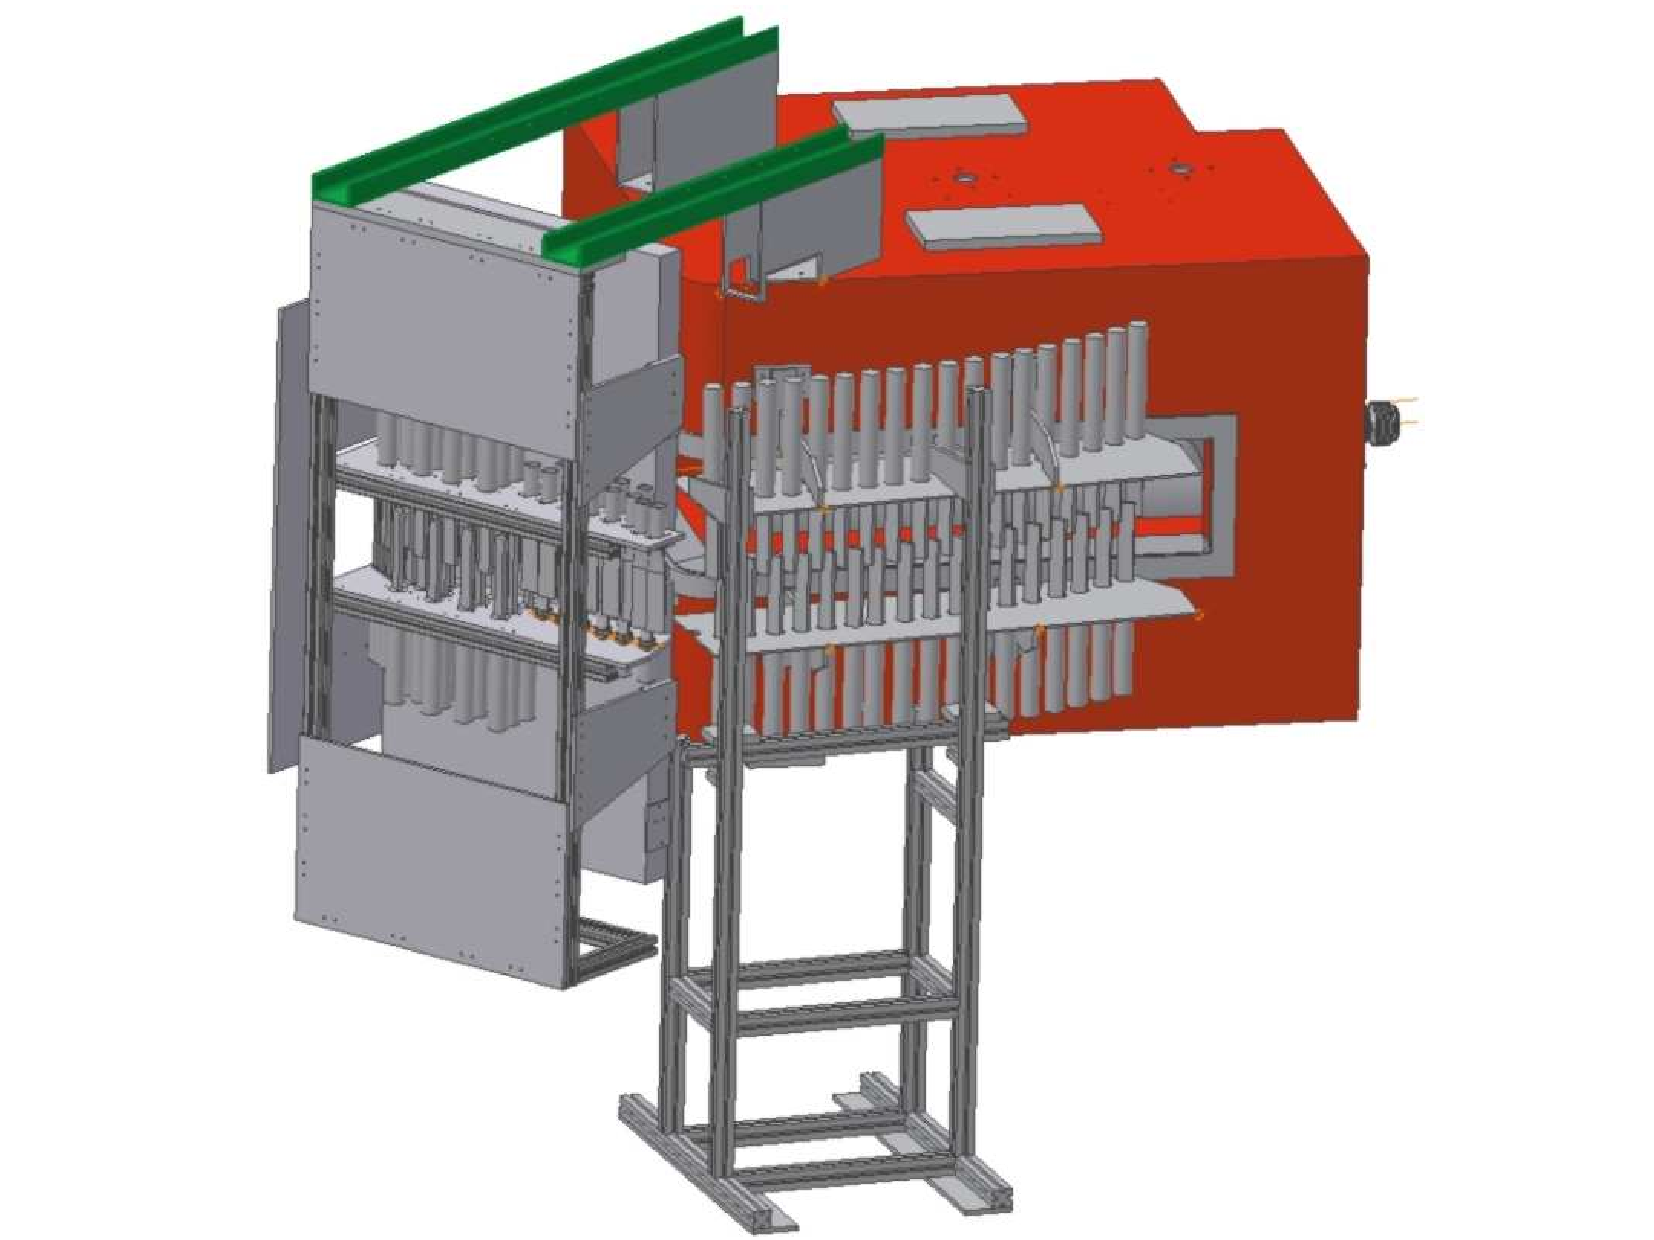
\includegraphics[width=\linewidth]{figs/Tagger.pdf}
	\caption{Top-down view of the tagging system consisting of dipole magnet (red) and scintillating bars and fibers \cite{tagger}. Electrons are deflected by the magnet after the bremsstrahlung process.}
	\label{fig:tagger}
\end{figure}
\end{minipage}
\section{Liquid hydrogen target}
\label{sec:tar}
The (polarized) photon beam impinges on a liquid hydrogen target \cite{hammannphd} which is located at the center of the crystal barrel detector, see Figure \ref{fig:cbarea}. It consists of a Kapton cell that measures $\SI{5.1}{\centi\m}$ in length and $\SI{3}{\centi\m}$ in diameter which is filled with liquid hydrogen. A separate cooling circuit with liquid hydrogen ensures the hydrogen that is used as target material stays liquid. Kapton is chosen as material for the target cell because the expected rate of hadronic reactions induced in the target cell is small compared to the expected rate from liquid hydrogen \cite{hammannphd}. Protons are bound with a binding energy of $\SI{21.4}{\eV}$ in the target material, which is negligible on the scale of hadronic reaction energies, so that they can be considered free. A schematic view of the target is shown in Figure \ref{fig:target}.
\begin{figure}[htbp]
	\centering
	\includegraphics[width=\linewidth]{figs/Target.pdf}
	\caption{Schematic overview of the liquid hydrogen target. Two tubes connected to a heat exchanger and the Kapton cell allow filling it with liquid hydrogen. \textsc{M. Grüner} in \cite{farahphd}.}
	\label{fig:target}
\end{figure}
\section{Detector system}
\label{sec:cal}
Hadronic reactions are induced by the photon beam in the target material. As a consequence resonances are excited that decay under emission of mesons. These mesons subsequently decay to e.g. photons. The main calorimeters of the experiment, the Crystal Barrel that is complemented by the forward detector(\ref{sec:cb}) and the MiniTAPS calorimeter (\ref{sec:mt}), cover $95\%$ of the solid angle $4\pi$ and are especially suited for the detection of photons. Charged particles are identified by the inner detector (\ref{sec:in}) as well as plastic scintillators mounted in front of the forward and the MiniTAPS detector that are used as vetoes. To suppress electromagnetic reactions a \textsc{\'Cerenkov} detector is used (\ref{sec:cerenkov}). The photon flux is measured via the Gamma-Intensity-Monitor (GIM) and Flux-Monitor (FluMo) (\ref{sec:flumo}).
\subsection{Inner detector}
\label{sec:in}
The inner detector \cite{indet,suft} encloses the target in a cylindrical geometry and consists of 513 plastic scintillation fibers that are placed in three layers. The outer layer is oriented along the beam axis while the inner layers are tilted by an angle of $\SI{-24.5}{\degree}$ and $\SI{25.8}{\degree}$, respectively, see Figure \ref{fig:indet}.
\begin{figure}[htbp]
	\centering
	
\includegraphics[width=\linewidth]{figs/indet.pdf}
	\caption{The inner detector with three layers of scintillating fibers. The inner two layers are tilted with respect to the outer layer. \textsc{D. Walther} in \cite{farahphd}.}
	\label{fig:indet}
\end{figure}
This structure allows to determine the azimuthal and polar angle of a charged particle as long as at least two layers are hit. The detector is in total $\SI{40}{\centi\meter}$ long and covers a polar angle range of $\SI{23.1}{\degree}<\theta<\SI{166}{\degree}$ with a resolution of $\SI{0.4}{\degree}$ in polar angle $\theta$ and $\SI{0.1}{\degree}$ in azimuthal angle $\phi$. The fibers consist of Polystyrene with a refractive index of $n=1.6$ and are cladded by Polymethylmetacrylat ($\text{C}_5\text{H}_8\text{O}_2$) with $n=1.49$ \cite{prop}. Charged particles passing the detector will cause the emission of scintillation light by the Polystyrene molecules which is read out with photomultipliers after passing lightguides. Short decay times ensure a fast time signal and a time resolution of $\text{FWHM}=\SI{2.093\pm0.013}{\nano\s}$ is reached \cite{hartmanndipl}.
\subsection{Crystal Barrel and forward detector}
\label{sec:cb}
\subsection{MiniTAPS}
\label{sec:mt}
\subsection{\textsc{\'Cerenkov} detector}
\label{sec:cerenkov}
\subsection{Flux monitoring}
\label{sec:flumo}
\begin{figure}[htbp]
	\centering
	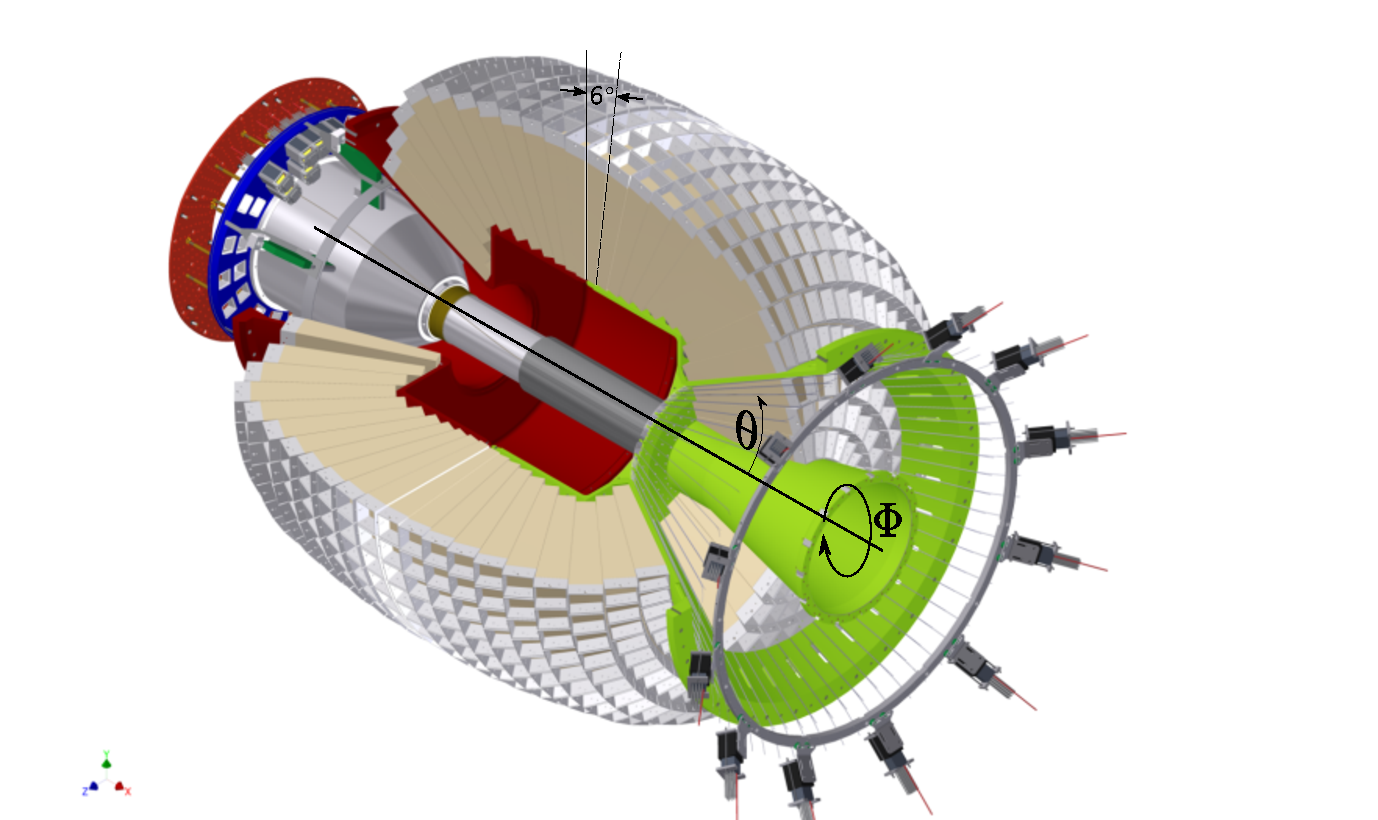
\includegraphics[width=\linewidth]{figs/cb_fp_in.pdf}
	\caption{\textsc{D. Walther} in \cite{urban}}
\end{figure}
\begin{figure}[htbp]
	\centering
	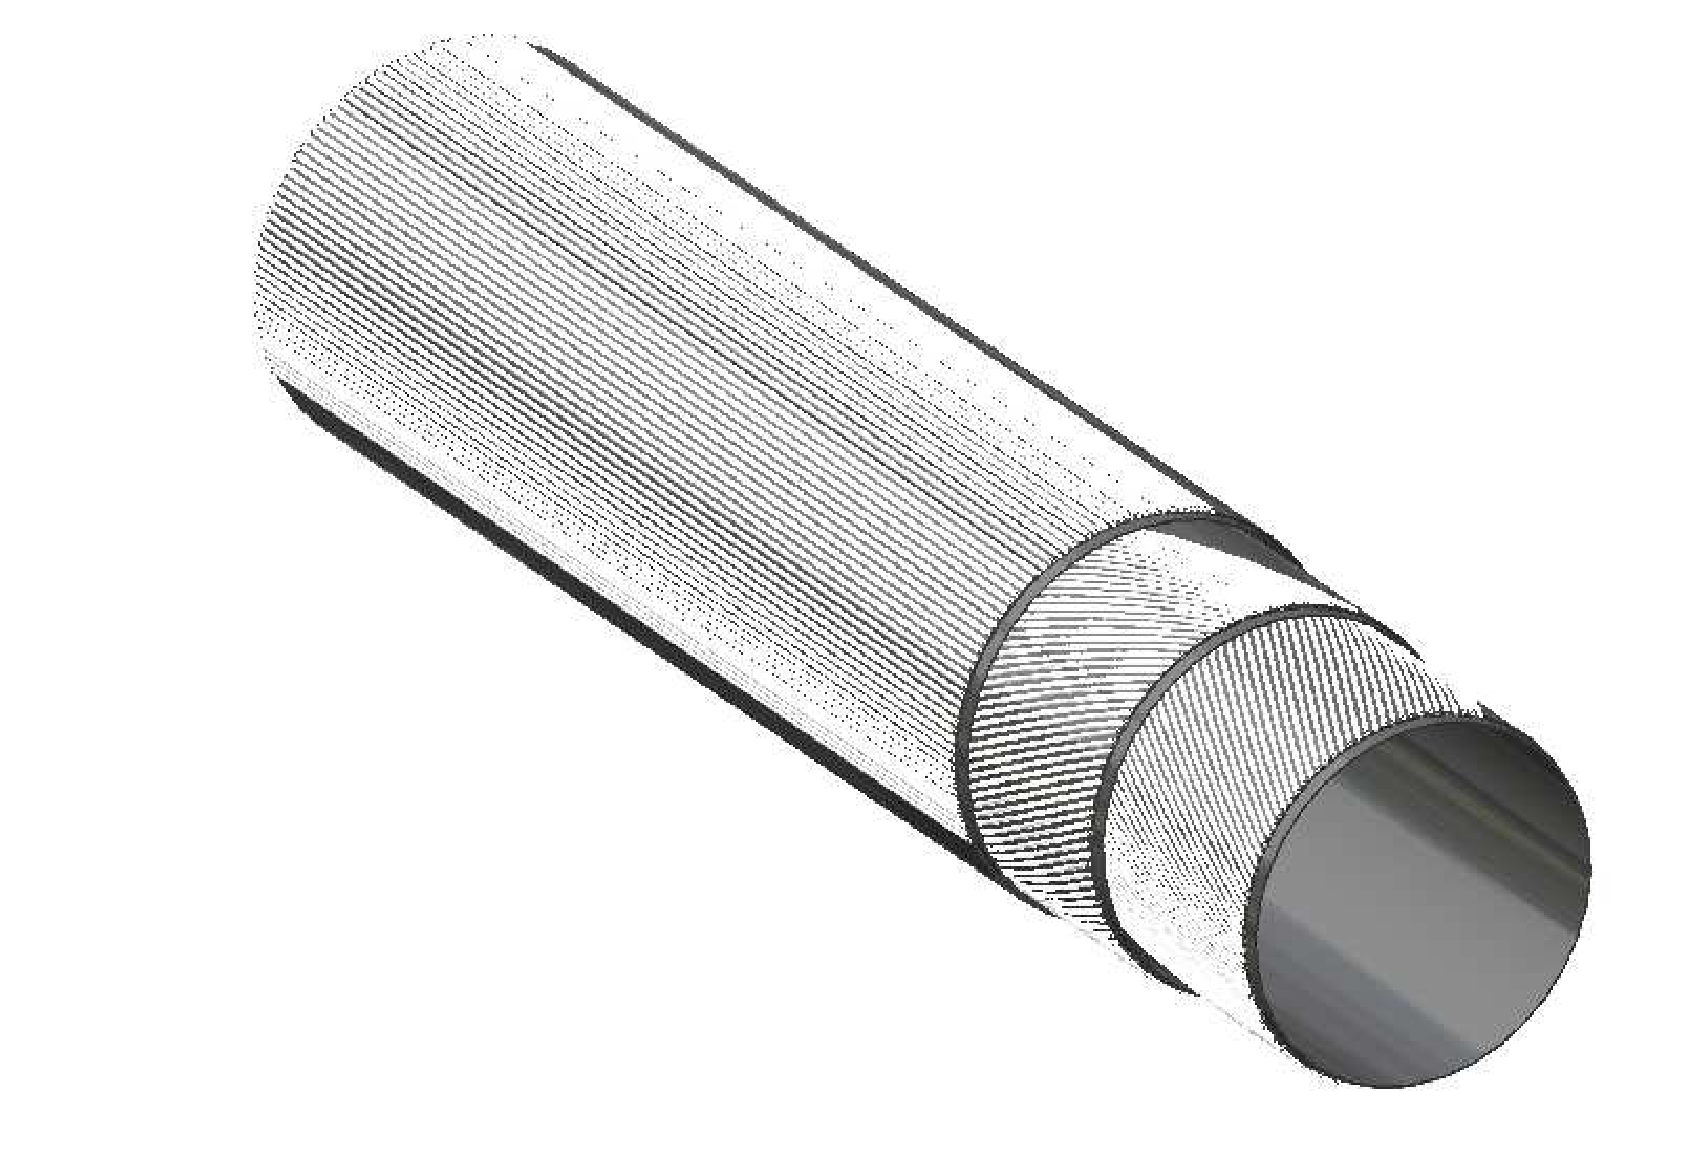
\includegraphics[width=.5\linewidth]{figs/faserorient.pdf}
	\caption{\cite{cb}}
\end{figure}
\begin{figure}[htbp]
	\centering
	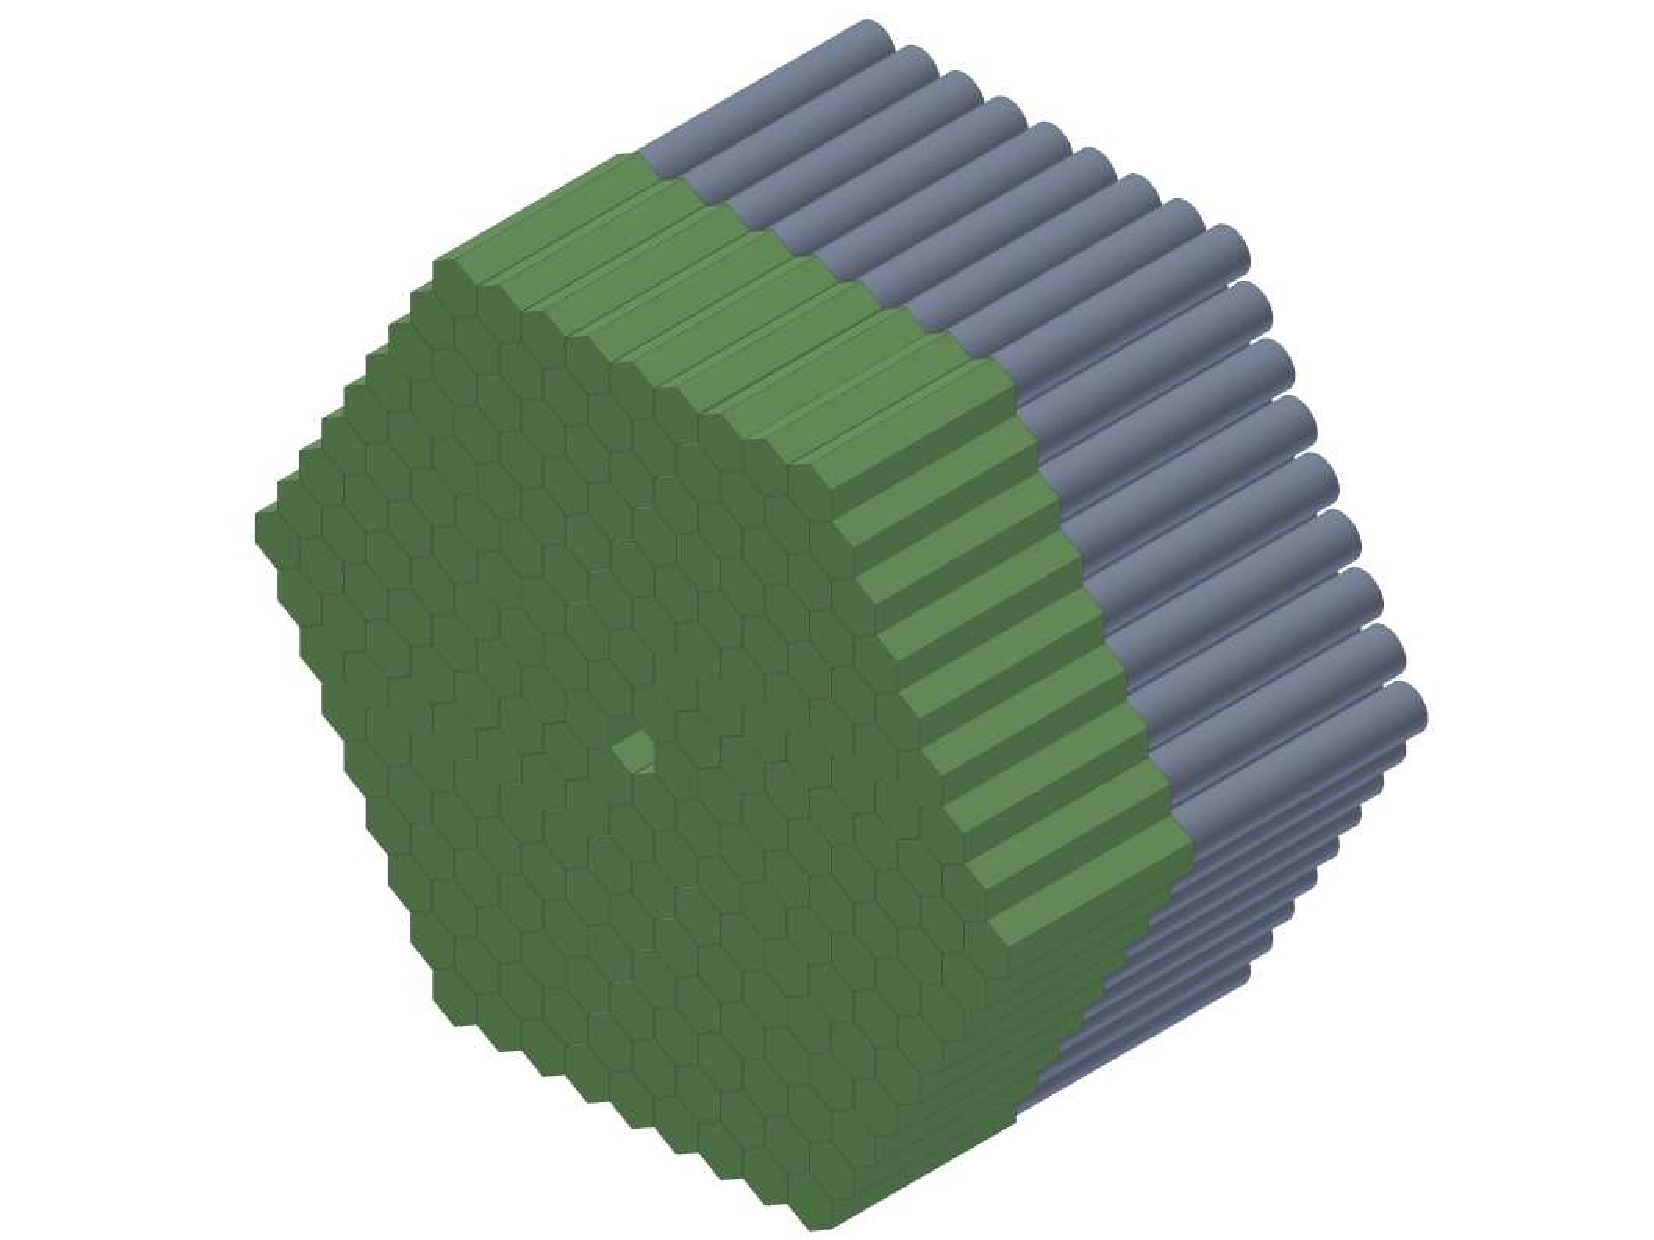
\includegraphics[width=.5\linewidth]{figs/mini-taps.pdf}
	\caption{\cite{cb}}
\end{figure}

\section{Trigger}
\label{sec:trig}

\section{Software and Monte Carlo}
\label{sec:mc}
\section{Datasets}